\begin{center}
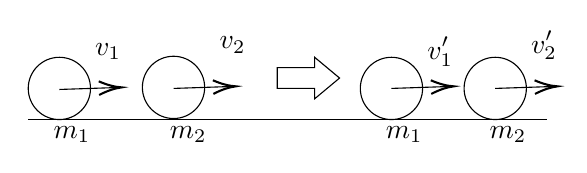
\begin{tikzpicture}[x=0.75pt,y=0.75pt,yscale=-1,xscale=1]
%uncomment if require: \path (0,300); %set diagram left start at 0, and has height of 300
%Straight Lines [id:da5712311460225725] 
\draw    (100,110) -- (350,110) ;
%Shape: Circle [id:dp501626887330255] 
\draw   (100,95) .. controls (100,86.72) and (106.72,80) .. (115,80) .. controls (123.28,80) and (130,86.72) .. (130,95) .. controls (130,103.28) and (123.28,110) .. (115,110) .. controls (106.72,110) and (100,103.28) .. (100,95) -- cycle ;
%Shape: Circle [id:dp8027430983175681] 
\draw   (155,94.5) .. controls (155,86.22) and (161.72,79.5) .. (170,79.5) .. controls (178.28,79.5) and (185,86.22) .. (185,94.5) .. controls (185,102.78) and (178.28,109.5) .. (170,109.5) .. controls (161.72,109.5) and (155,102.78) .. (155,94.5) -- cycle ;
%Shape: Circle [id:dp23940754387998542] 
\draw   (310,95) .. controls (310,86.72) and (316.72,80) .. (325,80) .. controls (333.28,80) and (340,86.72) .. (340,95) .. controls (340,103.28) and (333.28,110) .. (325,110) .. controls (316.72,110) and (310,103.28) .. (310,95) -- cycle ;
%Shape: Circle [id:dp9006459635140887] 
\draw   (260,95) .. controls (260,86.72) and (266.72,80) .. (275,80) .. controls (283.28,80) and (290,86.72) .. (290,95) .. controls (290,103.28) and (283.28,110) .. (275,110) .. controls (266.72,110) and (260,103.28) .. (260,95) -- cycle ;
%Right Arrow [id:dp7037165842832618] 
\draw   (220,85) -- (238,85) -- (238,80) -- (250,90) -- (238,100) -- (238,95) -- (220,95) -- cycle ;
%Straight Lines [id:da3133909490523399] 
\draw    (115,95.5) -- (143,94.57) ;
\draw [shift={(145,94.5)}, rotate = 178.09] [color={rgb, 255:red, 0; green, 0; blue, 0 }  ][line width=0.75]    (10.93,-3.29) .. controls (6.95,-1.4) and (3.31,-0.3) .. (0,0) .. controls (3.31,0.3) and (6.95,1.4) .. (10.93,3.29)   ;
%Straight Lines [id:da03685629638481602] 
\draw    (170,95) -- (198,94.07) ;
\draw [shift={(200,94)}, rotate = 178.09] [color={rgb, 255:red, 0; green, 0; blue, 0 }  ][line width=0.75]    (10.93,-3.29) .. controls (6.95,-1.4) and (3.31,-0.3) .. (0,0) .. controls (3.31,0.3) and (6.95,1.4) .. (10.93,3.29)   ;
%Straight Lines [id:da15780397999919527] 
\draw    (275,95) -- (303,94.07) ;
\draw [shift={(305,94)}, rotate = 178.09] [color={rgb, 255:red, 0; green, 0; blue, 0 }  ][line width=0.75]    (10.93,-3.29) .. controls (6.95,-1.4) and (3.31,-0.3) .. (0,0) .. controls (3.31,0.3) and (6.95,1.4) .. (10.93,3.29)   ;
%Straight Lines [id:da1252447585559464] 
\draw    (325,95) -- (353,94.07) ;
\draw [shift={(355,94)}, rotate = 178.09] [color={rgb, 255:red, 0; green, 0; blue, 0 }  ][line width=0.75]    (10.93,-3.29) .. controls (6.95,-1.4) and (3.31,-0.3) .. (0,0) .. controls (3.31,0.3) and (6.95,1.4) .. (10.93,3.29)   ;

% Text Node
\draw (111,112) node [anchor=north west][inner sep=0.75pt]   [align=left] {$\displaystyle m_{1}$};
% Text Node
\draw (167,112) node [anchor=north west][inner sep=0.75pt]   [align=left] {$\displaystyle m_{2}$};
% Text Node
\draw (271,112) node [anchor=north west][inner sep=0.75pt]   [align=left] {$\displaystyle m_{1}$};
% Text Node
\draw (321,112) node [anchor=north west][inner sep=0.75pt]   [align=left] {$\displaystyle m_{2}$};
% Text Node
\draw (131,72) node [anchor=north west][inner sep=0.75pt]   [align=left] {$\displaystyle v_{1}$};
% Text Node
\draw (191,69) node [anchor=north west][inner sep=0.75pt]   [align=left] {$\displaystyle v_{2}$};
% Text Node
\draw (291,69) node [anchor=north west][inner sep=0.75pt]   [align=left] {$\displaystyle v_{1}^{\prime }$};
% Text Node
\draw (341,66) node [anchor=north west][inner sep=0.75pt]   [align=left] {$\displaystyle v_{2}^{\prime }$};
\end{tikzpicture}
\end{center}